Depois de implementada a base de dados e o modo de comunicação entre cliente e servidor, podemos resumir o tráfego presente no nosso sistema com a Figura \ref{fig:trafego}.

\begin{figure}[H]
\centering
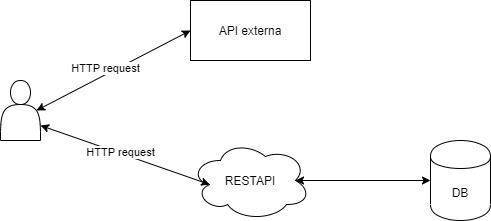
\includegraphics[width=0.5\linewidth]{images/DiagramaComunicacao.jpg}
\caption{Tráfego do Sistema.}
\label{fig:trafego}
\end{figure}